\documentclass[journal,12pt,onecolumn]{IEEEtran}
\usepackage[utf8]{inputenc}   % Codificación de entrada
\usepackage[T1]{fontenc}      % Codificación de fuente
\usepackage[spanish,es-tabla]{babel}   % Idioma español
\usepackage{lmodern}          % Fuente moderna
\usepackage{amsmath, amssymb} % Matemáticas y símbolos
\usepackage{graphicx} 		  % Gráficos e imágenes
\graphicspath{{img/}{tablas/}{portada/}}  % Las imágenes se buscarán en la carpeta "img"
\usepackage{longtable}      % Para tablas que se extienden en varias páginas
\usepackage{tabularx}	% Tablas avanzadas
\usepackage{threeparttable}
\usepackage{hyperref}	% Hipervínculos

%-------------------------------------------
% Otros paquetes útiles (personaliza según tus necesidades)
%-------------------------------------------
\usepackage{caption}
\usepackage{subcaption}
\usepackage{xcolor}
\usepackage{setspace}

%-------------------------------------------
% Comandos personalizados
\renewcommand{\listtablename}{Índice de tablas}
\renewcommand{\appendixname}{Anexos}
\definecolor{colorreferences}{RGB}{48,134,3}

% Metadatos del PDF
\hypersetup{
	unicode=true,
	hidelinks,
	colorlinks=true,       % false: boxed links; true: colored links
	linkcolor=black,          % color of internal links (change box color with linkbordercolor)
	citecolor=colorreferences,        % color of links to bibliography
	filecolor=magenta,      % color of file links
	urlcolor=blue,           % color of external links
	linkbordercolor={0 0 0}
}
%-------------------------------------------
% Inicio del documento
%-------------------------------------------

\begin{document}

% Aquí se encuentra el archivo con la portada
\begin{titlepage}
	\centering
	%-------------------------------------------
	% Logos en una tabla: izquierda, centro y derecha
	\begin{tabular}{@{}p{0.3\textwidth} p{0.3\textwidth} p{0.3\textwidth}@{}}
		
\includegraphics[height=2cm]{tecnm} & 
		\centering 
\includegraphics[height=1.5cm]{SEP} & 
		\raggedleft 
\includegraphics[height=2cm]{ith.jpg} \\
	\end{tabular}
	
	\vspace{2em}
	
	\noindent
	%-------------------------------------------
	%	Información institucional y académica (esquina superior izquierda)
	\begin{minipage}[t]{0.48\textwidth}
		\raggedright
		\small \textbf{%
			Instituto Tecnológico de Hermosillo\\
			Materia: Robótica\\
			Profesor: Medina Gil Lamadrid, Jesús Iván%
		}
	\end{minipage}%
	\hfill
	%	fecha actual (esquina superior derecha), en letras pequeñas y en negrita.
	\begin{minipage}[t]{0.48\textwidth}
		\raggedleft
		\small \textbf{\today}
	\end{minipage}
	
	\vspace{2em}
	
	%-----------------------------------------
	% Unidad y Título de la tarea en letras grandes y en negrita
	{\large \textbf{Unidad 1: Morfología del robot}}\\
	{\Huge \textbf{Tipos de Sensores
}}
		
	\vspace{1em}
	
	%---------------------------------------
	% Tabla con la información del equipo
	%---------------------------------------
	% Encabezado del equipo
	\begin{center}
		{\Large \textbf{Equipo 2}}
	\end{center}
	
	\vspace{1em}
	
	% Tabla de integrantes:
	% Cada fila contiene: foto (columna izquierda) y datos del integrante (columna derecha)
	\begin{center}
		\begin{tabular}{c c}
			\begin{tabular}{c}
				
\includegraphics[height=3cm]{perfil1.jpg} \\
				\textbf{Encinas Clark},\\ Efrain Adrian \\ \texttt{l21330568@hermosillo.tecnm.mx} \\ 
			\end{tabular} &
			\begin{tabular}{c}
				
\includegraphics[height=3cm]{perfil2.jpg} \\
				\textbf{Arredondo Solano,}\\ Yairee Daniela \\ \texttt{21330531@hermosillo.tecnm.mx} \\ 
			\end{tabular} \\ \vspace{2em}
			\begin{tabular}{c}
				
\includegraphics[height=3cm]{perfil3.jpg} \\
				\textbf{Vasquez Romero,}\\ Diego Jesus \\ \texttt{21330708@hermosillo.tecnm.mx} \\ 
			\end{tabular} &
			\begin{tabular}{c}
				
\includegraphics[height=3cm]{perfil4.jpg} \\
				\textbf{Cancio Elizondo ,}\\ Valeria Alejandra \\ \texttt{21330545@hermosillo.tecnm.mx} \\
			\end{tabular}
		\end{tabular}
	\end{center}

\end{titlepage}

%	Es innecesario poner el índice porque ya aparece en los marcadores del PDF
%\tableofcontents

% Ejemplo de inclusión de una sección (por ejemplo, "introduccion.tex" debe estar en la carpeta "secciones" y se recomienda no usar carácteres especiales (tilde) o espacios)

\section{Ejercicio 1}
\vspace{10mm}
\textbf{Por posición:}
\vspace{5mm}

\textbf{Encoder Incremental :} 

Este tipo de sensor óptico digital convierte el movimiento en una secuencia de pulsos digitales. Tiene una escala transparente con una retícula opaca; de un lado, tiene una escala equipada con una fuente de luz y un lente condensador. Del otro lado, hay celdas sensibles a la luz. La manera en la que funciona es que la resistencia de las celdas disminuye cada vez que reciben un rayo de luz, de este modo se genera un pulso cada vez que un rayo de luz es atravesado.


\begin{figure}[h]
	\centering
	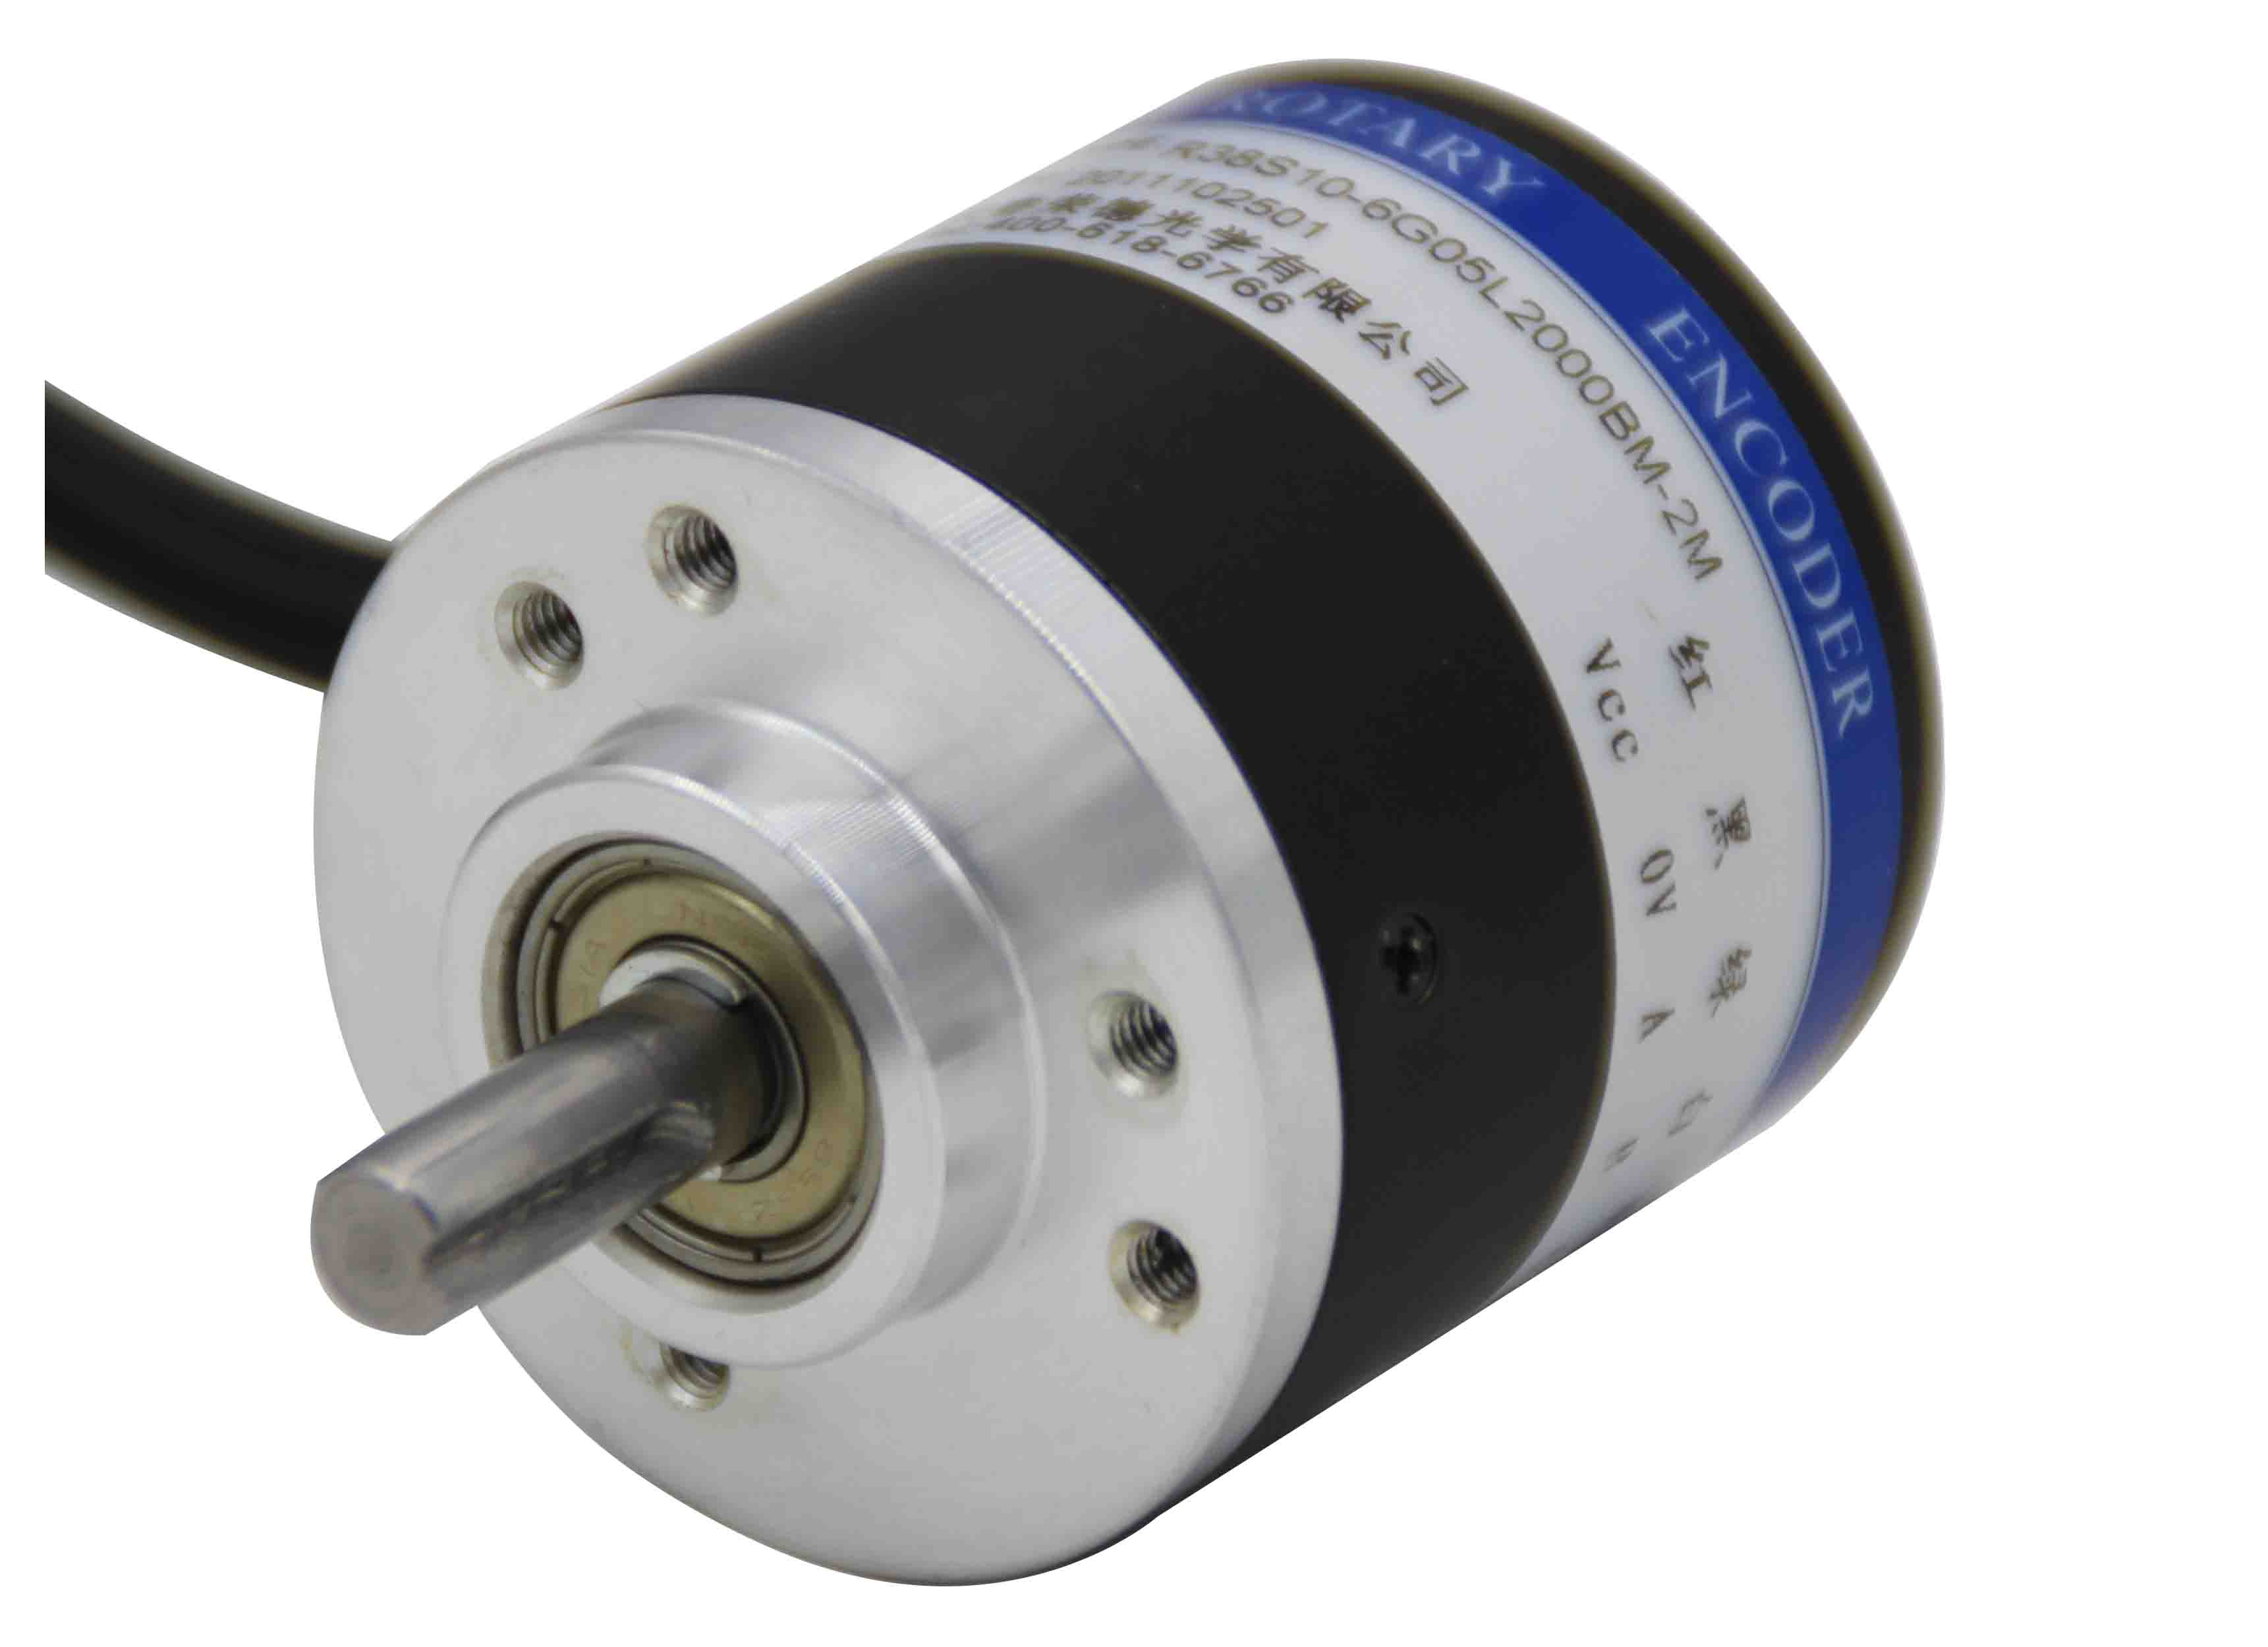
\includegraphics[width=0.4\linewidth]{portada/20150317193931229}
	\caption{Encoder incremental}
	\label{fig:20150317193931229}
\end{figure}

\begin{figure}[h]
	\centering
	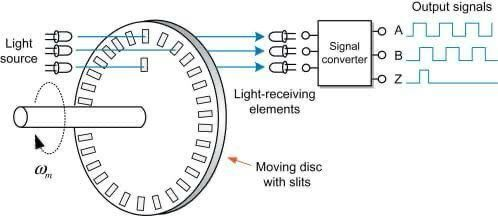
\includegraphics[width=0.4\linewidth]{img/Sencoderincremental}
	\caption{Codificador rotatorio incremental - OMCH}
	\label{fig:Sencoderincremental}
\end{figure}
\vspace{10mm}
\textbf{Encoder Absoluto :} 

Un encoder absoluto proporciona un valor único de posición en cualquier momento y permite que el sistema recuerde su ubicación incluso después de apagarse y encenderse nuevamente. Genera mensajes digitales que representan la posición actual del encoder, así como su velocidad y dirección de movimiento. En caso de pérdida de energía, su salida se corrige automáticamente al restablecer la alimentación, sin necesidad de regresar a una posición de referencia, como ocurre con los encoders incrementales.\\\\\\\\\\\\

\begin{figure}[h]
	\centering
	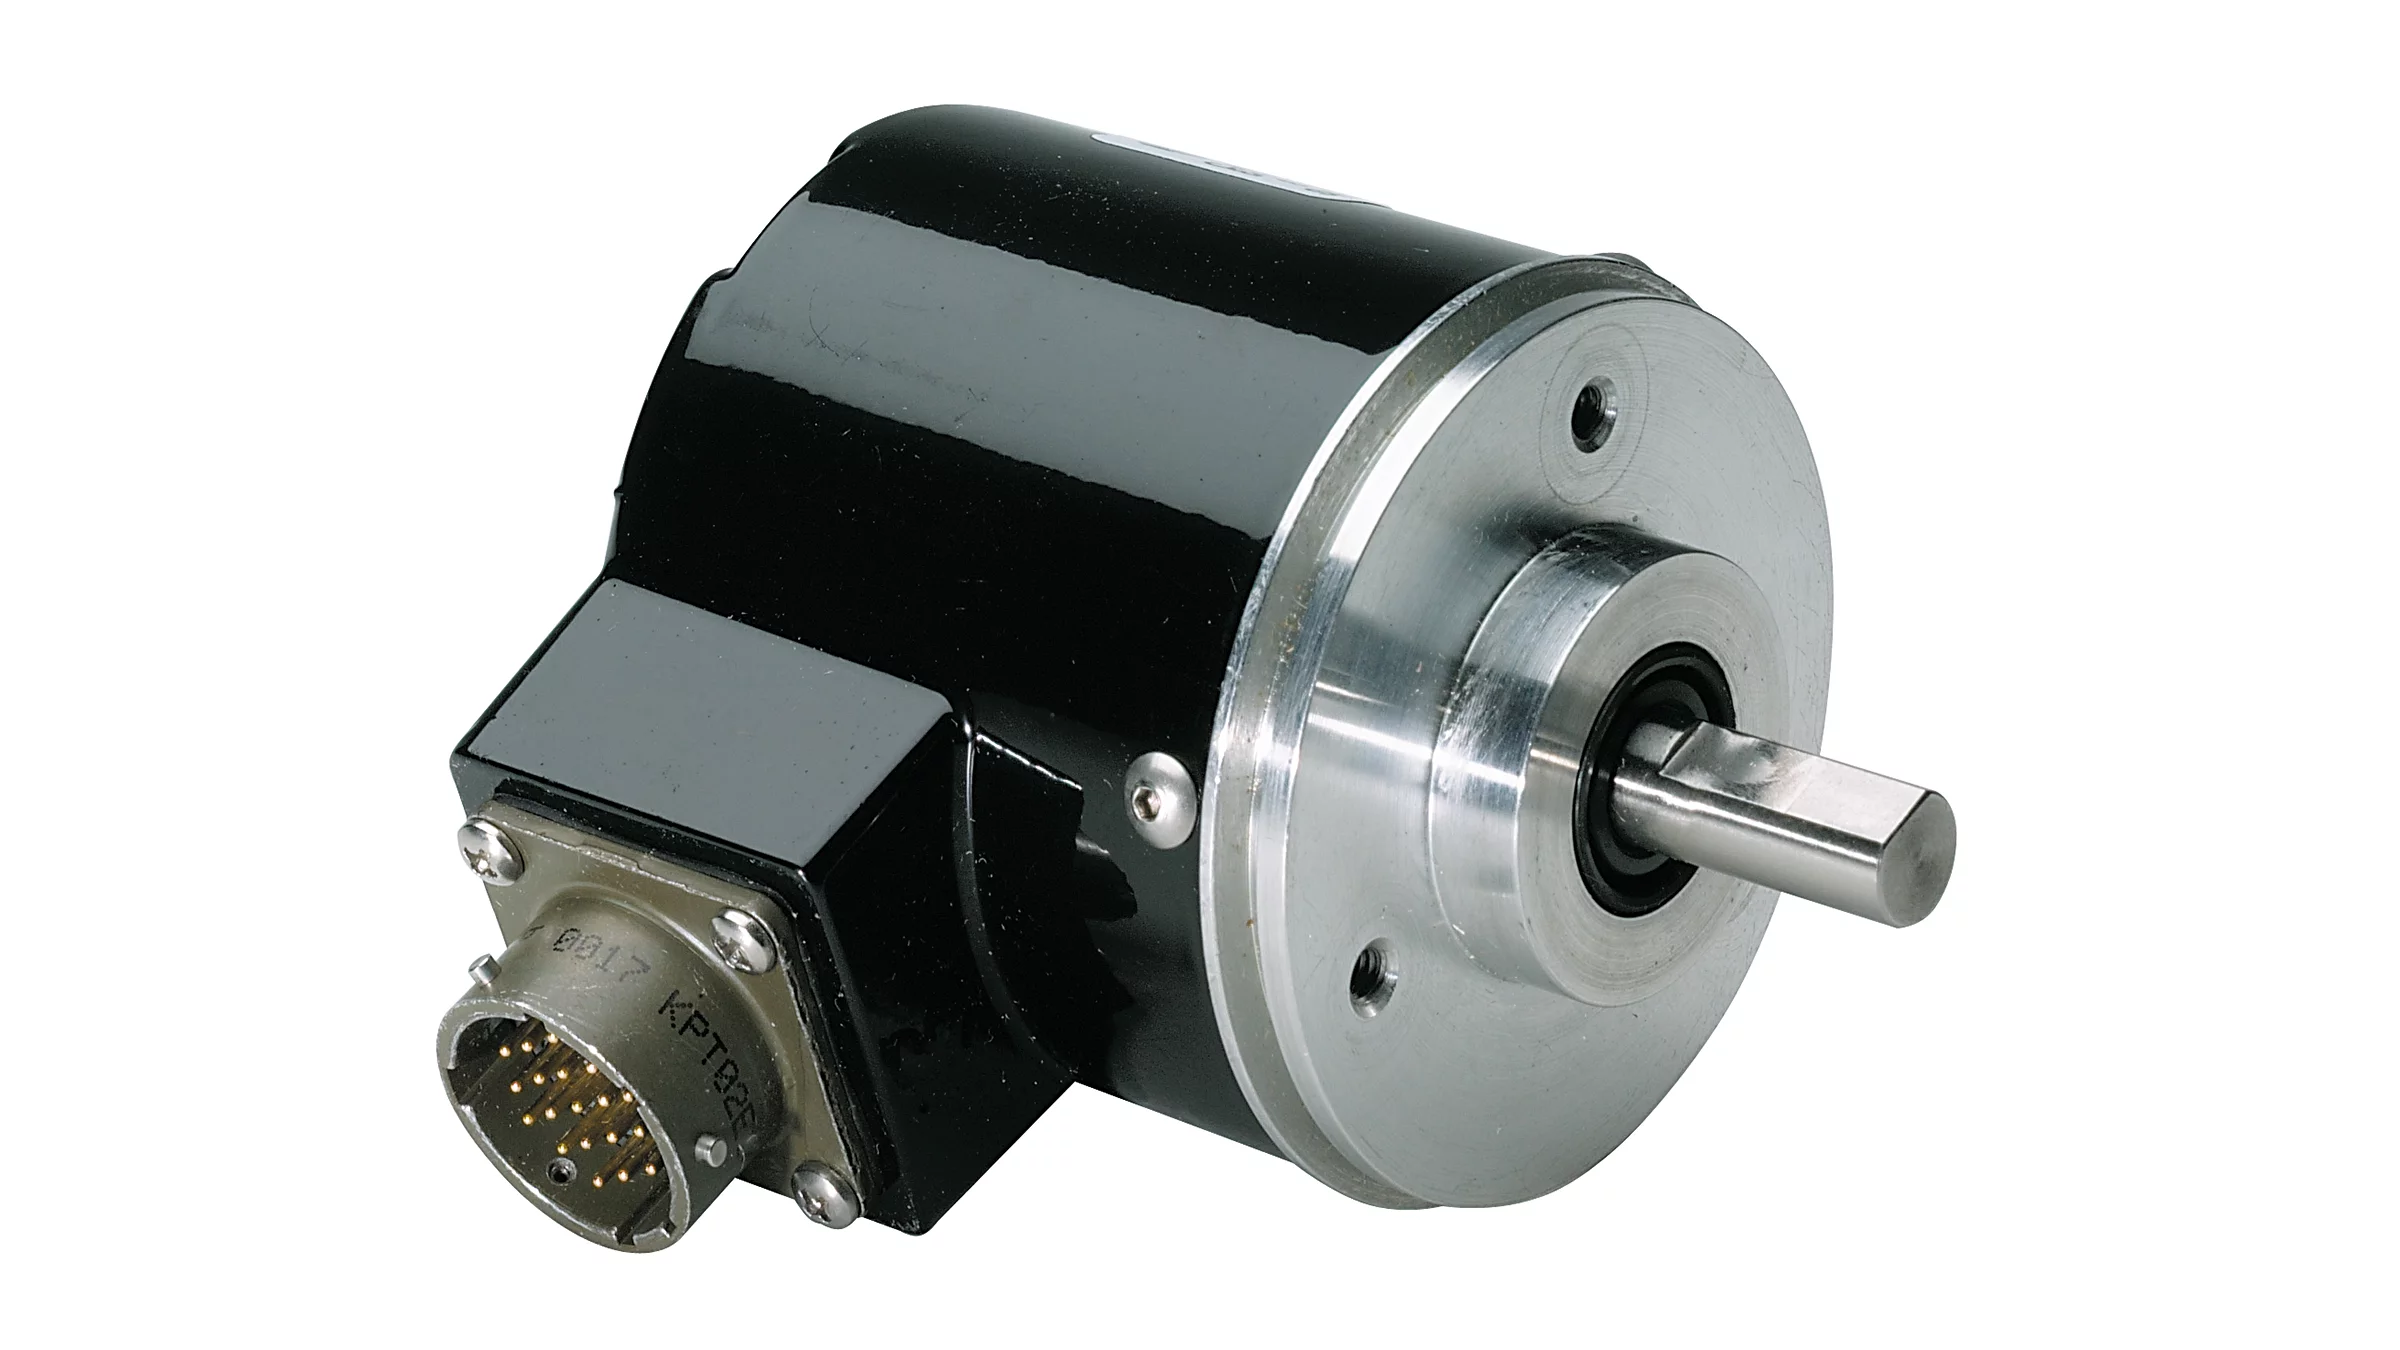
\includegraphics[width=0.4\linewidth, height=0.2\textwidth]{img/encoder}
	\caption{Encoder absoluto}
	\label{fig:encoder}
\end{figure} 

\begin{figure}[h]
	\centering
	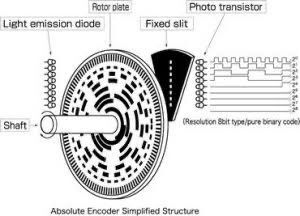
\includegraphics[width=0.4\linewidth]{img/Sencoderabsoluto}
	\caption{Funcionamiento de un encoder absoluto}
	\label{fig:Sencoderabsoluto}
\end{figure}

\vspace{10mm} 
% Párrafo de Potenciómetro
\textbf{Potenciómetro :} 

Es un dispositivo de resistencia variable que expresa desplazamientos lineales o angulares en términos de voltaje. Consiste en una clavija deslizante que hace contacto con un elemento resistivo, conforme se mueve este punto de contacto la resistencia entre el contacto deslizante y las conexiones de los extremos del dispositivo cambia en proporción al desplazamiento.


% Espacio para evitar que LaTeX mueva imágenes
\vspace{5mm}

% Primera imagen con su descripción
\begin{center}
	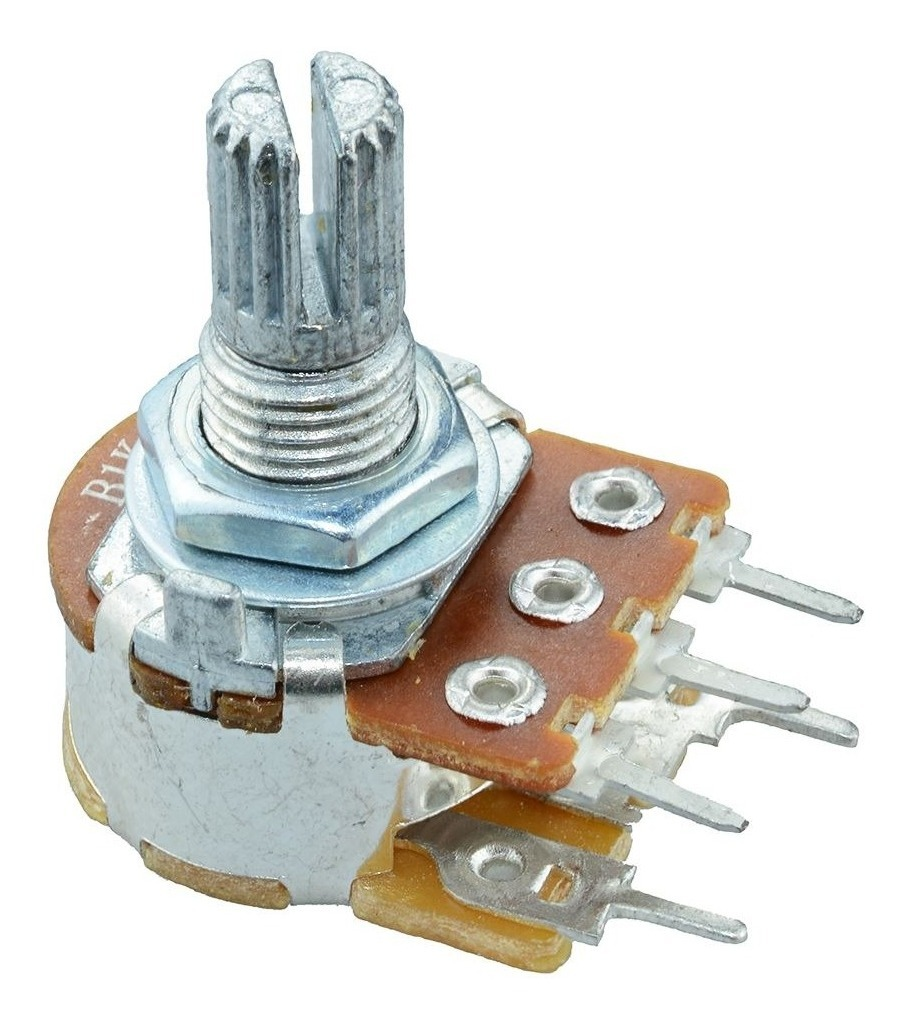
\includegraphics[width=0.3\linewidth]{img/potenciometro}
	
	\vspace{2mm} % Espacio entre imagen y descripción
	
	\textbf{Figura 5:} Potenciómetro
\end{center}

\vspace{5mm} % Espacio entre imágenes

% Segunda imagen con su descripción
\begin{center}
	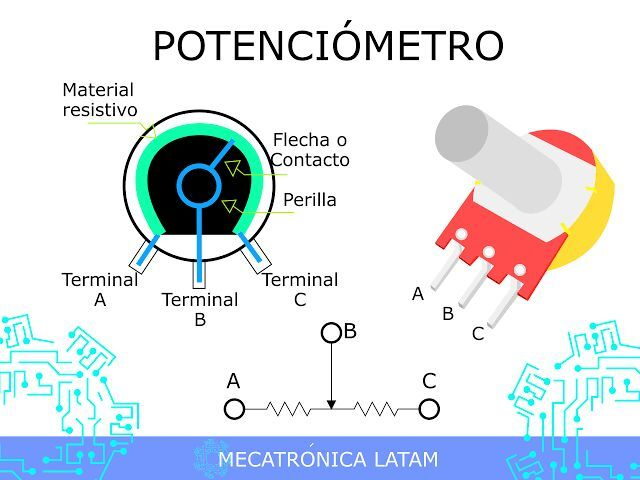
\includegraphics[width=0.4\linewidth]{img/Spotenciometro}
	
	\vspace{2mm} % Espacio entre imagen y descripción
	
	\textbf{Figura 6:} Diagrama de un potenciómetro.
\end{center}

\vspace{10mm}
\textbf{LVDT :} 

Es uno de los transductores de desplazamiento más populares ya que genera una señal de CA cuya magnitud se relaciona con el desplazamiento de un núcleo móvil. Tiene como concepto básico de un núcleo móvil rodeado por dos bobinas secundarias y una bobina principal y conforme el núcleo cambia su posición con respecto a las bobinas cambia también el campo magnético y por tanto se modifica la amplitud de voltaje en la bobina secundaria como una función del desplazamiento del núcleo a través de un segmento.

% Espacio para evitar que LaTeX mueva imágenes
\vspace{5mm}

% Primera imagen con su descripción
\begin{center}
	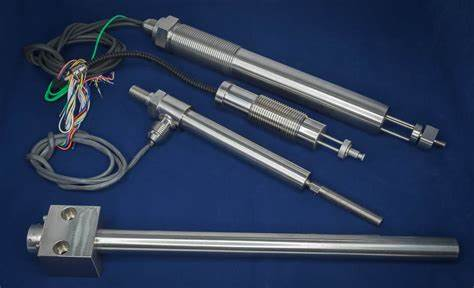
\includegraphics[width=0.3\linewidth]{img/LVDT}
	
	\vspace{2mm} % Espacio entre imagen y descripción
	
	\textbf{Figura 7:} LVDT
\end{center}

\vspace{5mm} % Espacio entre imágenes

% Segunda imagen con su descripción
\begin{center}
	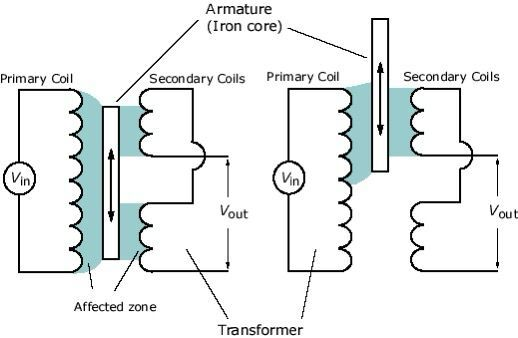
\includegraphics[width=0.5\linewidth]{img/Slvdt}
	
	\vspace{2mm} % Espacio entre imagen y descripción
	
	\textbf{Figura 8:} Funcionamiento de un LVDT.
\end{center}


\vspace{10mm}

% Párrafo de Resolver
\textbf{Resolver :} 

Son sensores que proporcionan señales análogas y consisten en un eje (flecha) solidario con una carcasa estacionaria. Sus señales deben ser convertidas en la forma digital por medio de un convertidor analógico a digital. Los resolvers tienen dos devanados orientados a 90°.

% Espacio para evitar que LaTeX mueva imágenes
\vspace{5mm}

% Primera imagen con su descripción
\begin{center}
	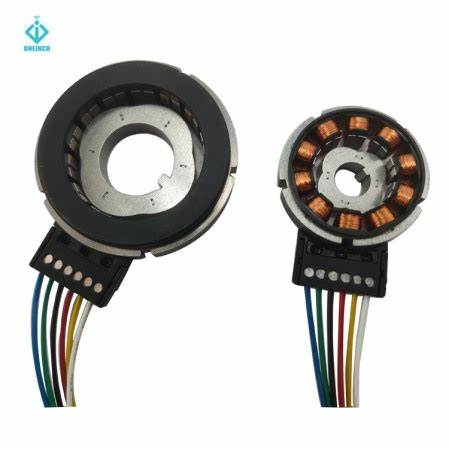
\includegraphics[width=0.2\linewidth, height=0.15\textheight]{img/resolver}
	
	\vspace{2mm} % Espacio entre imagen y descripción
	
	\textbf{Figura 9:} Resolver.
\end{center}

\vspace{5mm} % Espacio entre imágenes

% Segunda imagen con su descripción
\begin{center}
	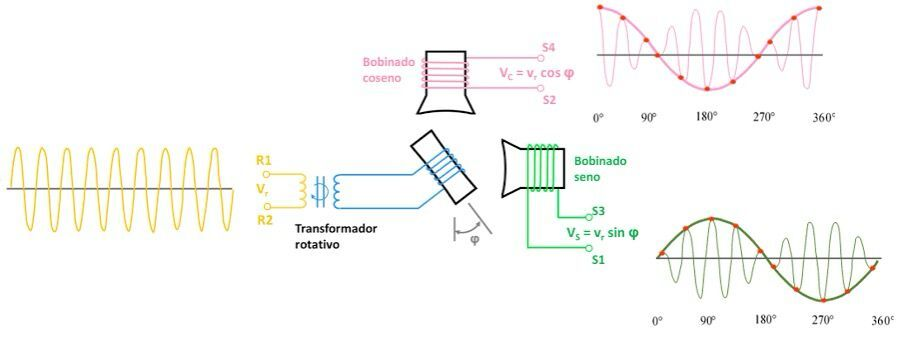
\includegraphics[width=0.4\linewidth]{img/Srevolver}
	
	\vspace{2mm} % Espacio entre imagen y descripción
	
	\textbf{Figura 10:} Funcionamiento de un resolver.
\end{center}

% Asegura que el siguiente párrafo no se junte con las imágenes
\vspace{10mm}



\textbf{Velocidad-tacogeneratriz :}

La captación de la velocidad se hace necesaria para mejorar el comportamiento dinámico de los actuadores del robot. La velocidad de movimiento de cada actuador (que tras el reductor es la velocidad de la articulación) se realimenta normalmente a un bucle de control analógico implementado en el propio accionador del elemento motor. No obstante, en ocasiones en las que el sistema de control del robot lo exija, la velocidad de giro de cada actuador es llevada hasta la unidad de control del robot. Normalmente, y puesto que el bucle de control de velocidad es analógico, el captador usado es una tacogeneratriz que proporciona una tensión proporcional a la velocidad de giro de su eje (valores típicos pueden ser 10 milivoltios por rpm). Otra posibilidad, usada para el caso de que la unidad de control del robot precise valorar la velocidad de giro de las articulaciones, consiste en derivar la información de posición que ésta posee.



% Espacio para evitar que LaTeX mueva imágenes
\vspace{5mm}

% Primera imagen con su descripción
\begin{center}
	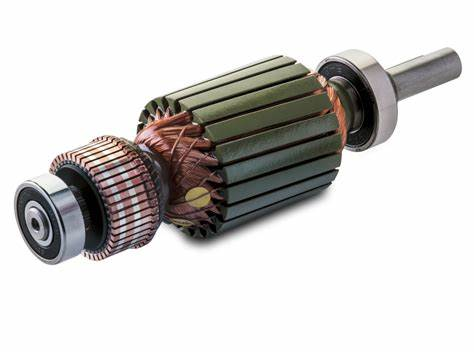
\includegraphics[width=0.3\linewidth]{img/OIP}
	
	\vspace{2mm} % Espacio entre imagen y descripción
	
	\textbf{Figura 11:} OIP
\end{center}

\vspace{5mm} % Espacio entre imágenes

% Segunda imagen con su descripción
\begin{center}
	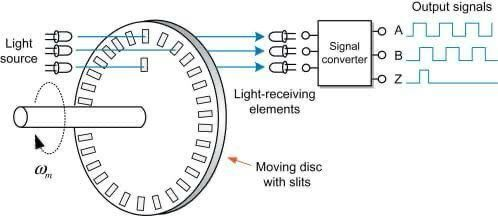
\includegraphics[width=0.5\linewidth]{img/Sencoderincremental}
	
	\vspace{2mm} % Espacio entre imagen y descripción
	
	\textbf{Figura 12:} Funcionamiento de un encoder incremental.
\end{center}

\vspace{10mm}
\textbf{Tacometro:}

Estos sensores pueden encontrar directamente la velocidad en cualquier momento ya que estos miden la velocidad de rotación de un elemento. Su diseño se basa en la regla de Fleming que declara que “el voltaje producido es proporcional al índice del acoplamiento inductivo”. Aquí un conductor (básicamente una bobina) se sujeta al elemento rotativo que gira en un campo magnético (estator). Conforme incrementa la velocidad del eje, el voltaje producido en las terminales de las bobinas también aumenta.

% Espacio para evitar que LaTeX mueva imágenes
\vspace{5mm}

% Primera imagen con su descripción
\begin{center}
	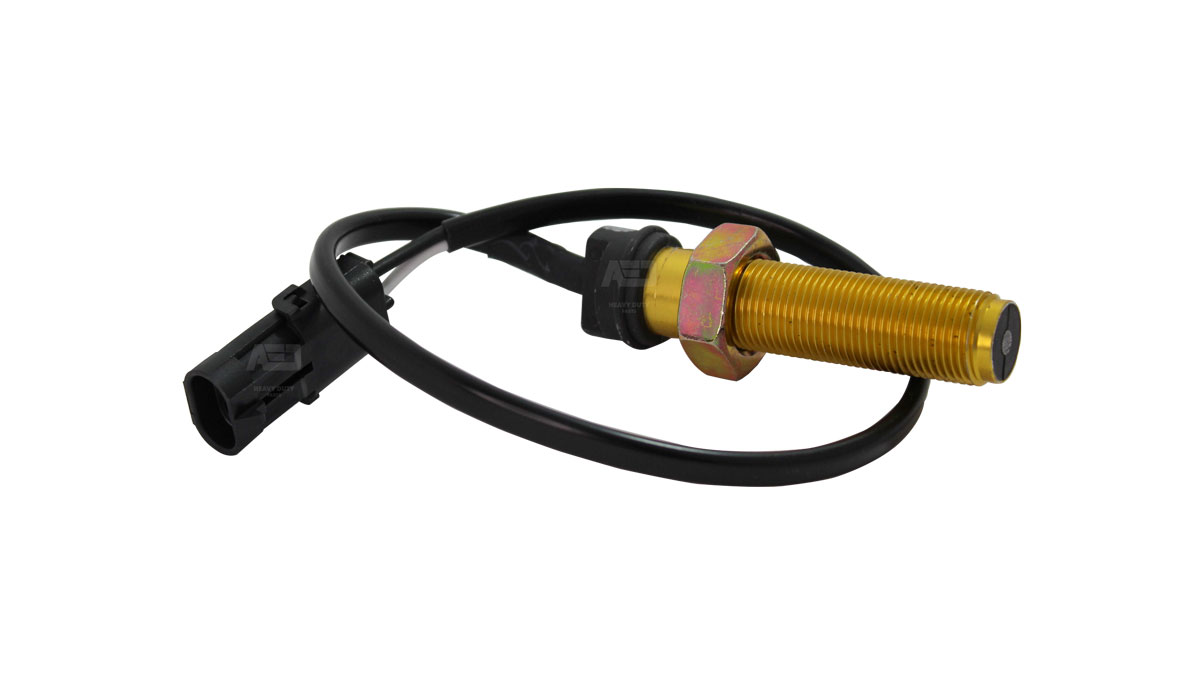
\includegraphics[width=0.5\linewidth, height=0.2\textheight]{img/tacometro}
	
	\vspace{2mm} % Espacio entre imagen y descripción
	
	\textbf{Figura 13:} Tacómetro.
\end{center}

\vspace{5mm} % Espacio entre imágenes

% Segunda imagen con su descripción
\begin{center}
	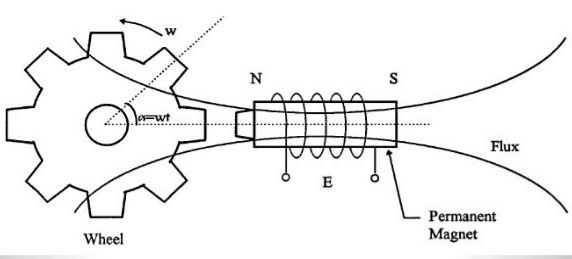
\includegraphics[width=0.7\linewidth]{img/Sveltaco}
	
	\vspace{2mm} % Espacio entre imagen y descripción
	
	\textbf{Figura 14:} Funcionamiento de un tacómetro.
\end{center}
\vspace{10mm}
\textbf{Sensor de Efecto Hall:}

Es un sensor de medición de velocidad el cual tiene el principio de “Si una pieza plana de material conductivo llamada chip Hall se sujeta a una diferencia de potencial en sus dos lados opuestos entonces el voltaje que se genera a través de las caras perpendiculares es cero”.

% Espacio para evitar que LaTeX mueva imágenes
\vspace{5mm}

% Primera imagen con su descripción
\begin{center}
	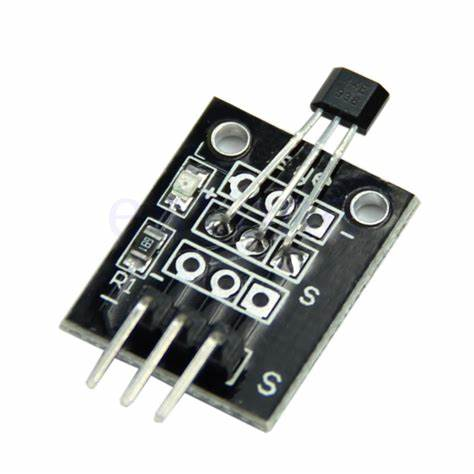
\includegraphics[width=0.1\linewidth, height=0.1\textheight]{img/HALL}
	
	\vspace{2mm} % Espacio entre imagen y descripción
	
	\textbf{Figura 15:} Sensor de efecto Hall.
\end{center}

\vspace{5mm} % Espacio entre imágenes

% Segunda imagen con su descripción
\begin{center}
	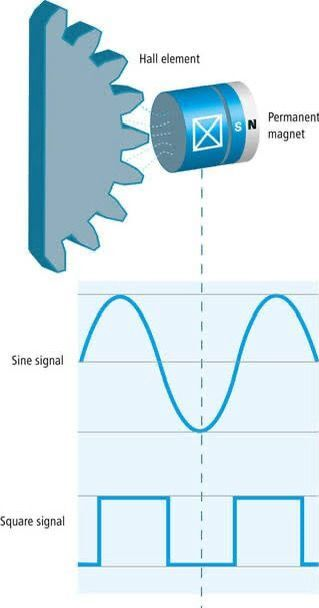
\includegraphics[width=0.3\linewidth]{img/Shall}
	
	\vspace{2mm} % Espacio entre imagen y descripción
	
	\textbf{Figura 16:} Funcionamiento de un sensor de efecto Hall.
\end{center}


\vspace{10mm}
\textbf{Galgas extensométricas:}

El principio de este sensor es que el alargamiento de un conductor aumenta su resistencia eléctrica. Este incremento de resistencia se debe a incremento de la longitud del conductor y decremento en el área del conductor.

% Espacio para evitar que LaTeX mueva imágenes
\vspace{5mm}

% Primera imagen con su descripción
\begin{center}
	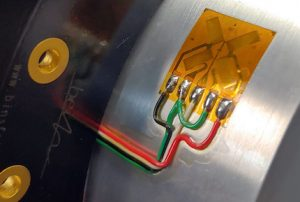
\includegraphics[width=0.3\linewidth, height=0.2\textheight]{img/galga-extensiometrica-300x202}
	
	\vspace{2mm} % Espacio entre imagen y descripción
	
	\textbf{Figura 17:} Galga extensiométrica.
\end{center}

\vspace{5mm} % Espacio entre imágenes

% Segunda imagen con su descripción
\begin{center}
	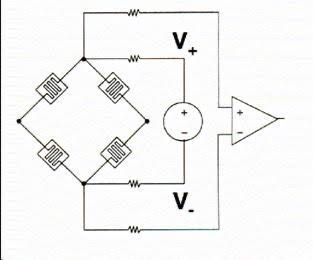
\includegraphics[width=0.5\linewidth]{img/Sgalgas}
	
	\vspace{2mm} % Espacio entre imagen y descripción
	
	\textbf{Figura 18:} Funcionamiento de galgas extensiométricas.
\end{center}

\vspace{10mm}
\textbf{Interruptores piezoeléctricos:}

Son sensores que utilizan un material piezoeléctrico el cual señala que cuando cristales eléctricos asimétricos se deforman mediante una fuerza, se desarrolla un potencial eléctrico dentro de la red cristalina deformada. Son capaces de medir fuerzas, presiones, vibraciones y aceleraciones.


% Espacio para evitar que LaTeX mueva imágenes
\vspace{5mm}

% Primera imagen con su descripción
\begin{center}
	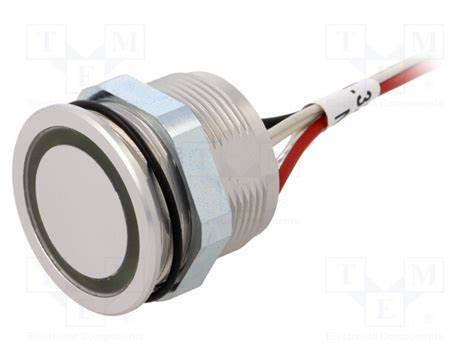
\includegraphics[width=0.3\linewidth, height=0.2\textheight]{img/S}
	
	\vspace{2mm} % Espacio entre imagen y descripción
	
	\textbf{Figura 19:} Sensor piezoeléctrico.
\end{center}

\vspace{5mm} % Espacio entre imágenes

% Segunda imagen con su descripción
\begin{center}
	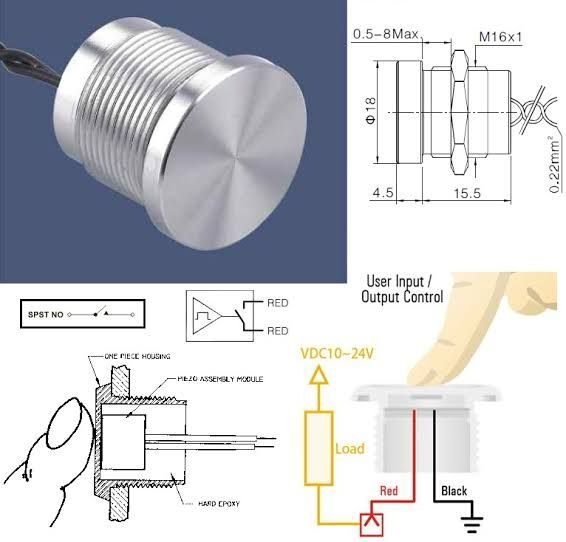
\includegraphics[width=0.5\linewidth]{img/Spiezoelectrico}
	
	\vspace{2mm} % Espacio entre imagen y descripción
	
	\textbf{Figura 20:} Funcionamiento de sensor piezoeléctrico.
\end{center}
\vspace{10mm}
\textbf{Tipo de contacto : }
\vspace{10mm}

\textbf{Interruptores de límite : }

Un interruptor de límite tiene un brazo mecánico sensible a la presión, y al momento  en el que un  objeto aplica presión en el brazo, se activa el interruptor.  Contiene un mecanismo de conmutación el cual su actuador activa el mecanismo que cierra o abre un circuito eléctrico. 
% Espacio para evitar que LaTeX mueva imágenes
\vspace{5mm}

% Primera imagen con su descripción
\begin{center}
	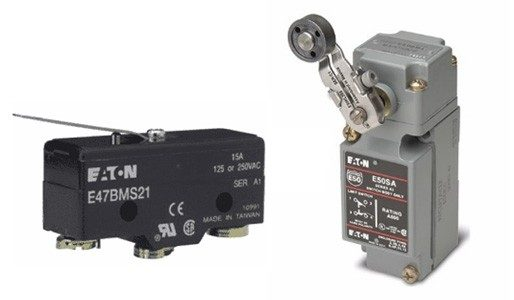
\includegraphics[width=0.4\linewidth, height=0.2\textwidth]{img/intlimite}
	
	\vspace{2mm} % Espacio entre imagen y descripción
	
	\textbf{Figura 21:} Interruptor de límite.
\end{center}

\vspace{5mm} % Espacio entre imágenes

% Segunda imagen con su descripción
\begin{center}
	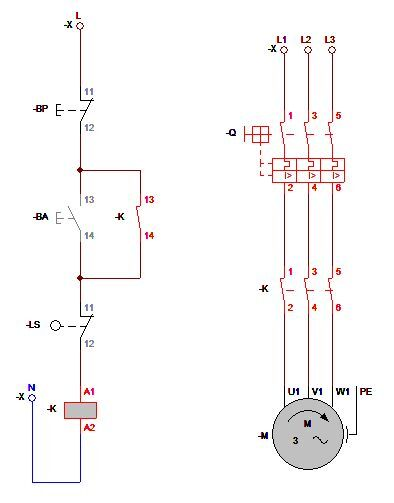
\includegraphics[width=0.4\linewidth]{img/Sinterruptordelimite}
	
	\vspace{2mm} % Espacio entre imagen y descripción
	
	\textbf{Figura 22:} Funcionamiento del interruptor de límite.
\end{center}


\vspace{10mm}
\textbf{Interruptores neumáticos : }

Son un tipo de dispositivo de conmutación que utiliza aire para funcionar. Al momento que se comprime el interruptor neumático envía un soplo a lo largo del tubo de PCV y llega a un interruptor de aire. El movimiento del aire activará el interruptor de aire, que creará el circuito eléctrico y activará un dispositivo.
% Espacio para evitar que LaTeX mueva imágenes
\vspace{5mm}

% Primera imagen con su descripción
\begin{center}
	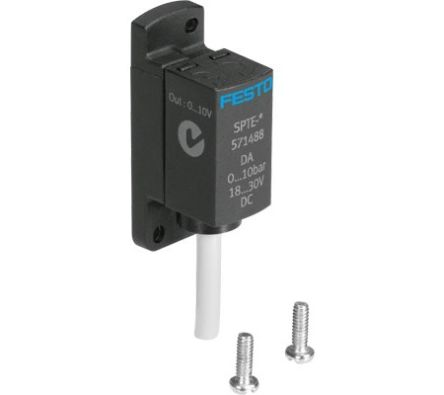
\includegraphics[width=0.4\linewidth, height=0.2\textwidth]{img/neumatico}
	
	\vspace{2mm} % Espacio entre imagen y descripción
	
	\textbf{Figura 23:} Interruptor neumático.
\end{center}

\vspace{5mm} % Espacio entre imágenes

% Segunda imagen con su descripción
\begin{center}
	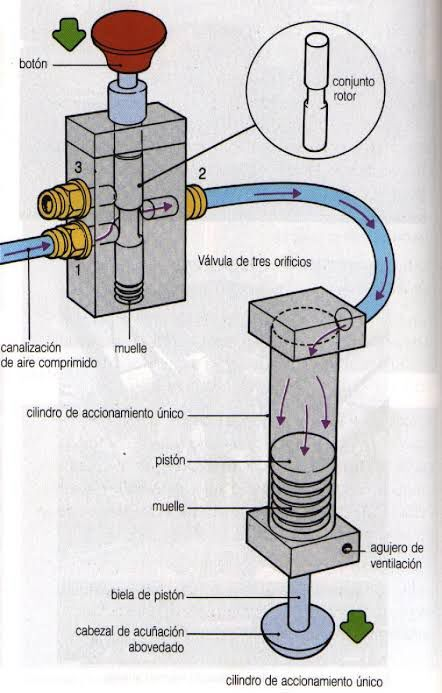
\includegraphics[width=0.4\linewidth]{img/Sinterruptorneumatico}
	
	\vspace{2mm} % Espacio entre imagen y descripción
	
	\textbf{Figura 24:} Funcionamiento del interruptor neumático.
\end{center}

\vspace{10mm}
\textbf{}
\textbf{Transductores de presión : }

Es un dispositivo que convierte la presión en una señal de salida eléctrica, esta puede ser digital o analógica y es utilizada por otros dispositivos como controladores, alarmas y otros sistemas de circuito cerrado. Estos dispositivos son cruciales para garantizar la seguridad y eficiencia en los sistemas al proporcionar datos de presión precisos. 


% Espacio para evitar que LaTeX mueva imágenes
\vspace{5mm}

% Primera imagen con su descripción
\begin{center}
	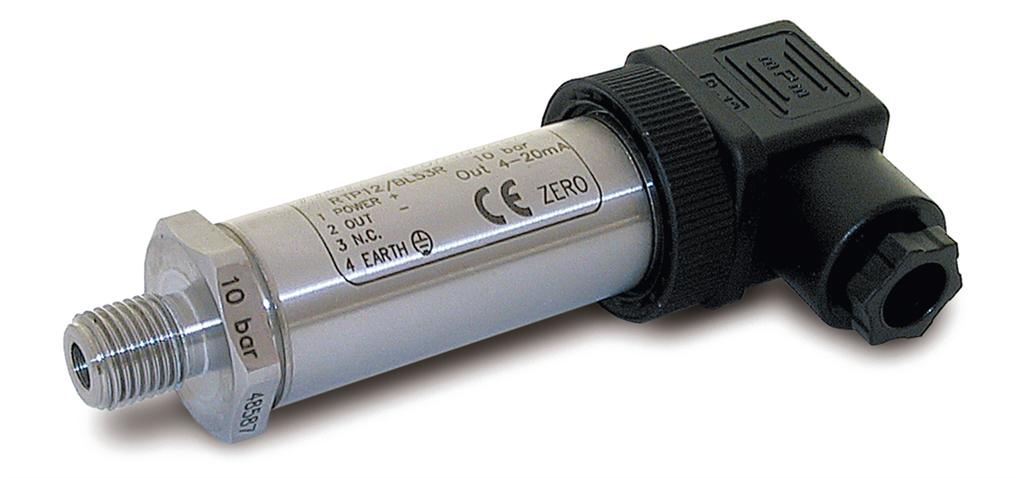
\includegraphics[width=0.4\linewidth, height=0.2\textwidth]{img/transductorpresion}
	
	\vspace{2mm} % Espacio entre imagen y descripción
	
	\textbf{Figura 25:} Transductor de presión
\end{center}

\vspace{5mm} % Espacio entre imágenes

% Segunda imagen con su descripción
\begin{center}
	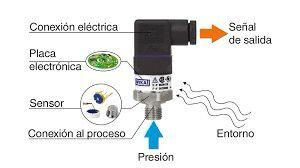
\includegraphics[width=0.4\linewidth]{img/Stransmisordepresion}
	
	\vspace{2mm} % Espacio entre imagen y descripción
	
	\textbf{Figura 26:} Funcionamiento de transductor de presión
\end{center}

\vspace{10mm}
\textbf{}
\textbf{Tipo sin contacto: }

\vspace{10mm}
\textbf{Sensores de proximidad : }

Existen dos tipos de sensores de proximidad : inductivo y capacitivo. Los sensores de proximidad inductivos se usan en lugar de interruptores de límite para la detección sin contacto de objetos metálicos. Los sensores de proximidad capacitivos se usan sobre la misma base que los sensores de proximidad inductivos, pero también pueden detectar objetos no metálicos.


% Espacio para evitar que LaTeX mueva imágenes
\vspace{5mm}

% Primera imagen con su descripción
\begin{center}
	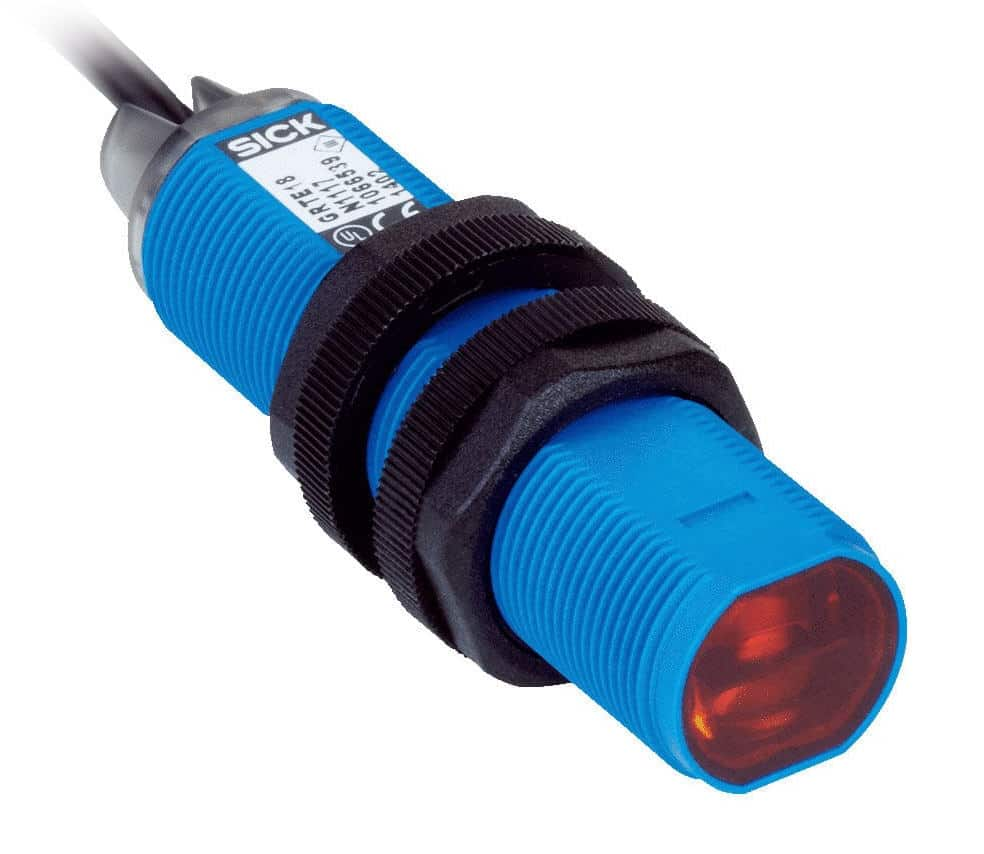
\includegraphics[width=0.4\linewidth, height=0.3\textwidth]{img/proximidad}
	
	\vspace{2mm} % Espacio entre imagen y descripción
	
	\textbf{Figura 27:} Sensor de proximidad
\end{center}

\vspace{5mm} % Espacio entre imágenes

% Segunda imagen con su descripción
\begin{center}
	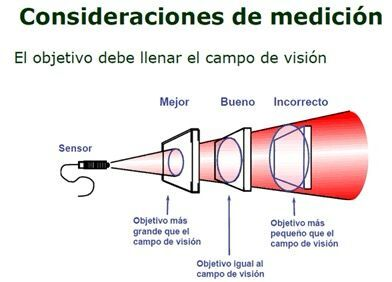
\includegraphics[width=0.4\linewidth]{img/Ssensorproximidad}
	
	\vspace{2mm} % Espacio entre imagen y descripción
	
	\textbf{Figura 28:} Funcionamiento de sensor de proximidad
\end{center}

\vspace{10mm}
\textbf{Sensores de microondas : }

Son sensores que utilizan la frecuencia de microondas para detectar el movimiento en una zona mediante la emisión de impulsos de microondas y la posterior medición del reflejo de un objeto en movimiento. Funcionan según el principio del efecto Doppler. Cuando la frecuencia de microondas emitida encuentra un objeto en movimiento en su campo de detección, la frecuencia de retorno se altera, indicando así el movimiento.

% Espacio para evitar que LaTeX mueva imágenes
\vspace{5mm}

% Primera imagen con su descripción
\begin{center}
	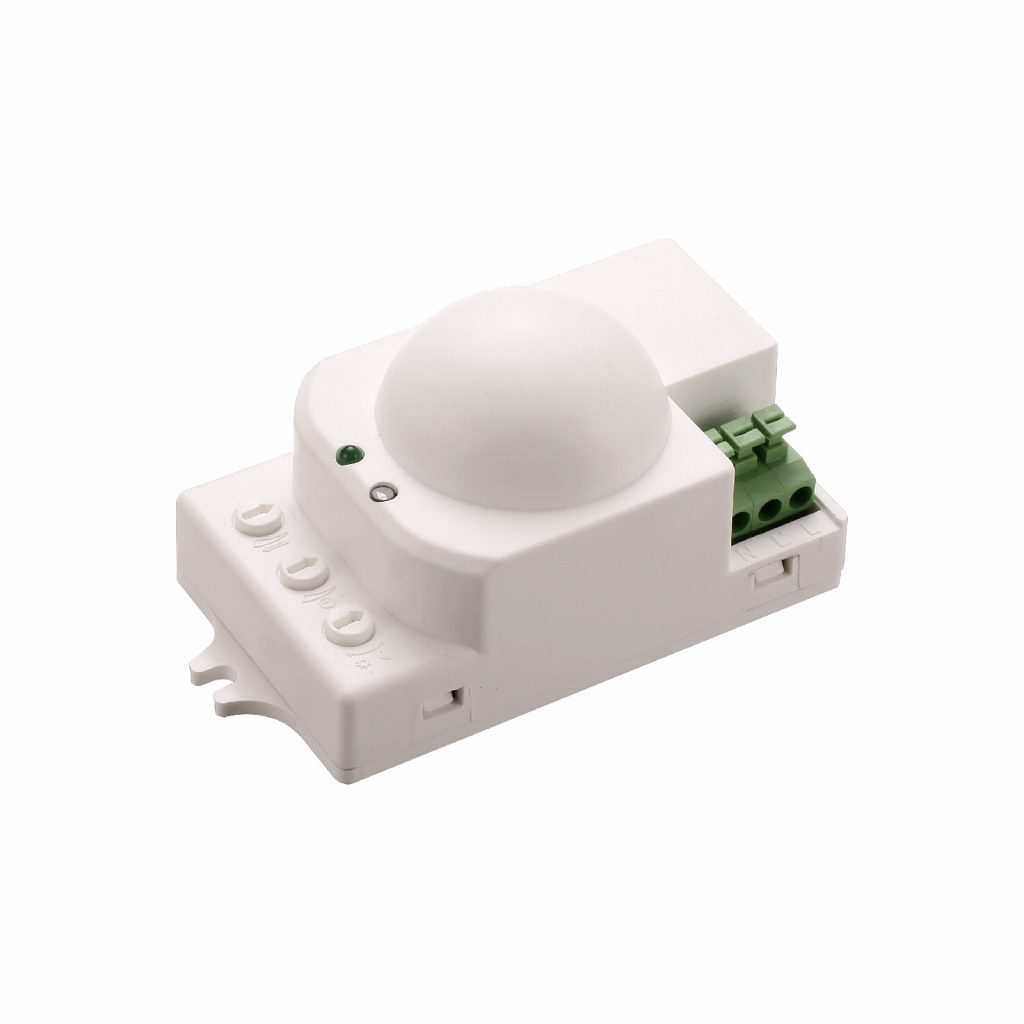
\includegraphics[width=0.4\linewidth, height=0.2\textwidth]{img/microondas}
	
	\vspace{2mm} % Espacio entre imagen y descripción
	
	\textbf{Figura 29:} Sensor de microondas
\end{center}

\vspace{5mm} % Espacio entre imágenes

% Segunda imagen con su descripción
\begin{center}
	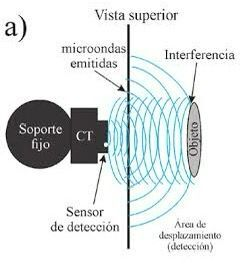
\includegraphics[width=0.4\linewidth]{img/Smicroondas}
	
	\vspace{2mm} % Espacio entre imagen y descripción
	
	\textbf{Figura 30:} Funcionamiento de sensor de microondas
\end{center}


\vspace{10mm}
\textbf{Sensores ultrasónicos : }

Son sensores los cuales miden la distancia mediante el uso de ondas ultrasónicas. Está formado por un cabezal el cual emite una onda ultrasónica y recibe la onda reflejada que retorna desde el objeto. Este tipo de sensores miden la distancia al objeto  contando el tiempo entre la emisión y la recepción. 


% Espacio para evitar que LaTeX mueva imágenes
\vspace{5mm}

% Primera imagen con su descripción
\begin{center}
	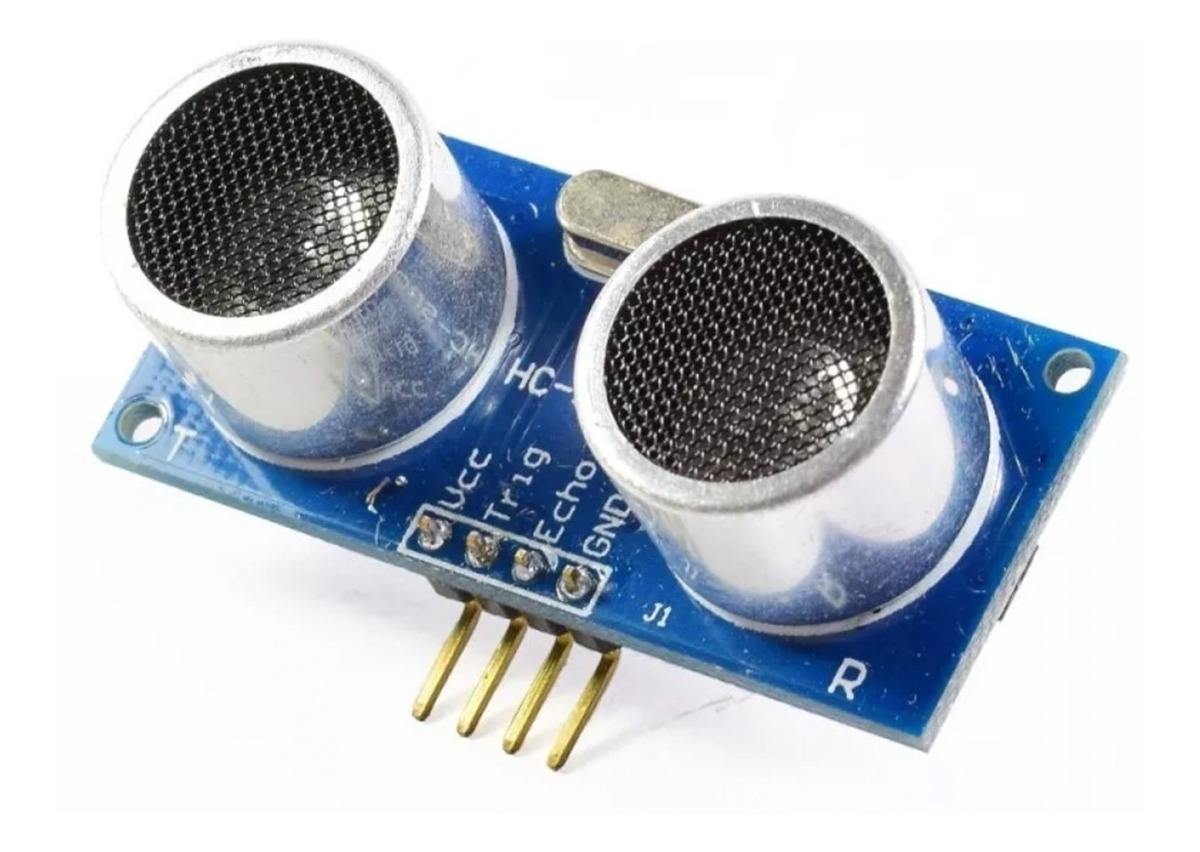
\includegraphics[width=0.4\linewidth, height=0.2\textwidth]{img/ultrasonido}
	
	\vspace{2mm} % Espacio entre imagen y descripción
	
	\textbf{Figura 31:} Sensor ultrasónico
\end{center}

\vspace{5mm} % Espacio entre imágenes

% Segunda imagen con su descripción
\begin{center}
	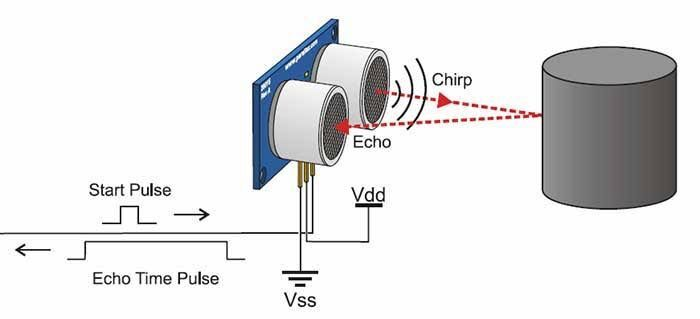
\includegraphics[width=0.5\linewidth]{img/Sultrasonicos}
	
	\vspace{2mm} % Espacio entre imagen y descripción
	
	\textbf{Figura 32:} Funcionamiento de sensor ultrasónico
\end{center}



\vspace{10mm}
\textbf{Sensores Láser : }

Este tipo de sensores utiliza un “laser” para lograr emitir luz en una línea recta. Su punto de haz visible hace que su alineación y posicionamiento sean sencillos. Este haz de luz es emitido desde el elemento emisor de luz en el transmisor y es recibido por el elemento de recepción de luz en el receptor. 
% Espacio para evitar que LaTeX mueva imágenes
\vspace{5mm}

% Primera imagen con su descripción
\begin{center}
	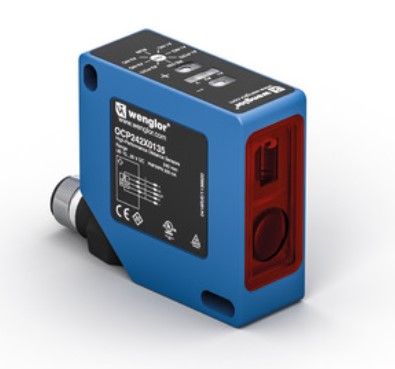
\includegraphics[width=0.4\linewidth, height=0.2\textwidth]{img/laser}
	
	\vspace{2mm} % Espacio entre imagen y descripción
	
	\textbf{Figura 33:} Sensor láser
\end{center}

\vspace{5mm} % Espacio entre imágenes

% Segunda imagen con su descripción
\begin{center}
	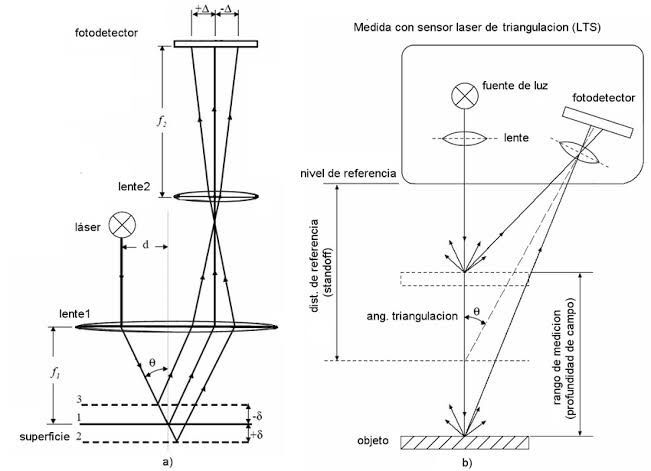
\includegraphics[width=0.4\linewidth]{img/Slaser}
	
	\vspace{2mm} % Espacio entre imagen y descripción
	
	\textbf{Figura 34:} Funcionamiento del sensor láser
\end{center}

\vspace{10mm}
\textbf{Sensor de visión : }

Estos sensores son un tipo de solución de visión artificial los cuales utilizan imágenes capturadas por una cámara para determinar la presencia, orientación y  precisión de las piezas. Estos sensores se diferencian de los “sistemas” de inspección de imagen, en que la cámara, la luz y el controlador están contenidos en una sola unidad, lo que simplifica la construcción y operación de la misma.

% Espacio para evitar que LaTeX mueva imágenes
\vspace{5mm}

% Primera imagen con su descripción
\begin{center}
	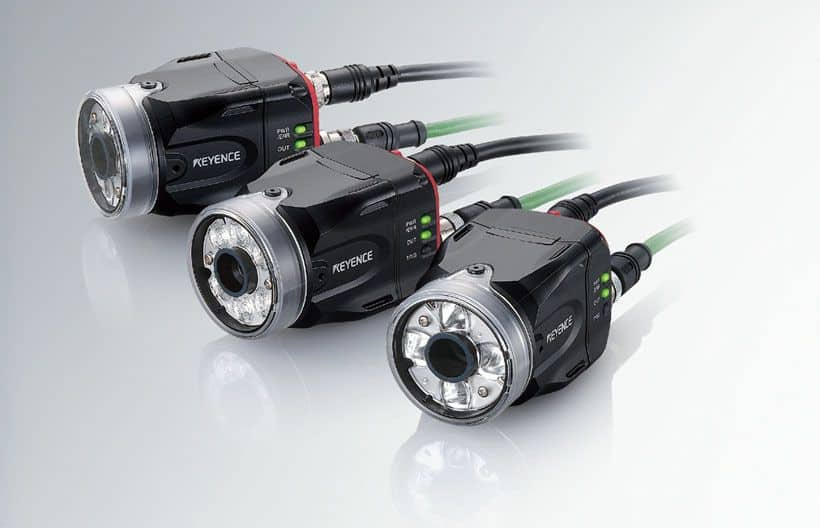
\includegraphics[width=0.4\linewidth, height=0.2\textwidth]{img/vision}
	
	\vspace{2mm} % Espacio entre imagen y descripción
	
	\textbf{Figura 35:} Sensor de visión
\end{center}

\vspace{5mm} % Espacio entre imágenes

% Segunda imagen con su descripción
\begin{center}
	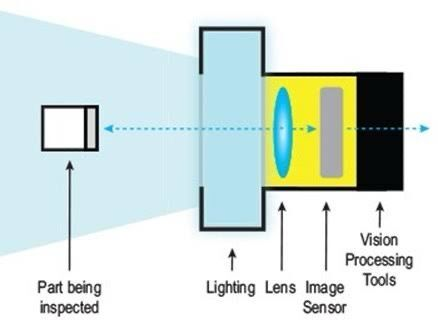
\includegraphics[width=0.5\linewidth]{img/Svision}
	
	\vspace{2mm} % Espacio entre imagen y descripción
	
	\textbf{Figura 36:} Funcionamiento del sensor de visión
\end{center}



\vspace{10mm}
\section{Adicionales}
\vspace{10mm}
\textbf{Giroscopio :}

Este tipo de sensores utiliza un “laser” para lograr emitir luz en una línea recta. Su punto de haz visible hace que su alineación y posicionamiento sean sencillos. Este haz de luz es emitido desde el elemento emisor de luz en el transmisor y es recibido por el elemento de recepción de luz en el receptor. 
\vspace{10mm}  % Espacio de 10 puntos



% Primera imagen con su descripción
\begin{center}
	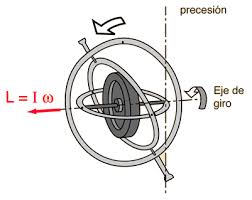
\includegraphics[width=0.3\linewidth, height=0.23\textheight]{img/giros}
	
	\vspace{2mm} % Espacio entre imagen y descripción
	
	\textbf{Figura 37:} Giroscopio
\end{center}

\vspace{5mm} % Espacio entre imágenes

% Segunda imagen con su descripción
\begin{center}
	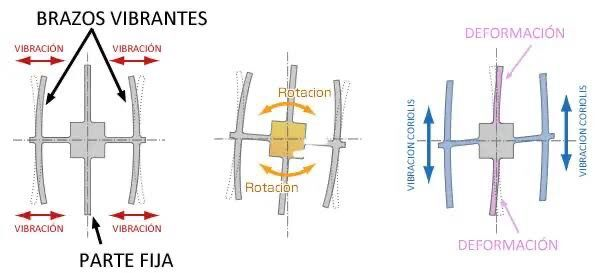
\includegraphics[width=0.6\linewidth]{img/Sgiroscopio}
	
	\vspace{2mm} % Espacio entre imagen y descripción
	
	\textbf{Figura 38:} Funcionamiento del giroscopio
\end{center}

\vspace{10mm}
\textbf{Acelerómetro :}

Un acelerómetro mide la aceleración a través del cambio en la capacitancia. Su estructura incluye una masa conectada a un resorte, permitiendo que se desplace en una dirección específica dentro de un marco con placas fijas. Cuando se aplica una aceleración, la masa se mueve, lo que modifica la capacitancia entre las placas y la masa. Este cambio es medido y procesado para determinar el valor de la aceleración correspondiente.


% Espacio para evitar que LaTeX mueva imágenes
\vspace{5mm}

% Primera imagen con su descripción
\begin{center}
	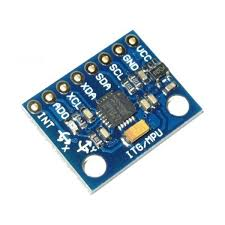
\includegraphics[width=0.2\linewidth, height=0.2\textheight]{img/acelerometro}
	
	\vspace{2mm} % Espacio entre imagen y descripción
	
	\textbf{Figura 39:} Acelerómetro
\end{center}

\vspace{5mm} % Espacio entre imágenes

% Segunda imagen con su descripción
\begin{center}
	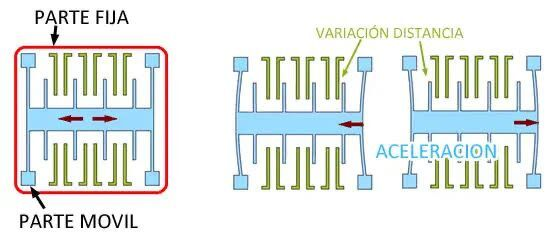
\includegraphics[width=0.6\linewidth]{img/Sacelerometro}
	
	\vspace{2mm} % Espacio entre imagen y descripción
	
	\textbf{Figura 40:} Funcionamiento del acelerómetro
\end{center}



\vspace{10mm}
\textbf{Magnetómetro :}

El magnetómetro detecta el campo magnético terrestre utilizando principalmente el efecto Hall o, en menor medida, el efecto magnetorresistivo. En la mayoría de los sensores del mercado, el efecto Hall funciona de la siguiente manera: si se aplica una corriente a través de una placa conductora, los electrones fluyen en línea recta. Sin embargo, la presencia de un campo magnético altera esta trayectoria, desviando los electrones hacia un lado de la placa y generando una diferencia de voltaje proporcional a la intensidad del campo. Por otro lado, los sensores que emplean el efecto magnetorresistivo utilizan materiales sensibles al magnetismo, como aleaciones de hierro y níquel. Cuando estos materiales son expuestos a un campo magnético, su resistencia eléctrica varía, permitiendo la medición del campo.
\vspace{10pt}  % Espacio de 10 puntos

% Espacio para evitar que LaTeX mueva imágenes
\vspace{5mm}

% Primera imagen con su descripción
\begin{center}
	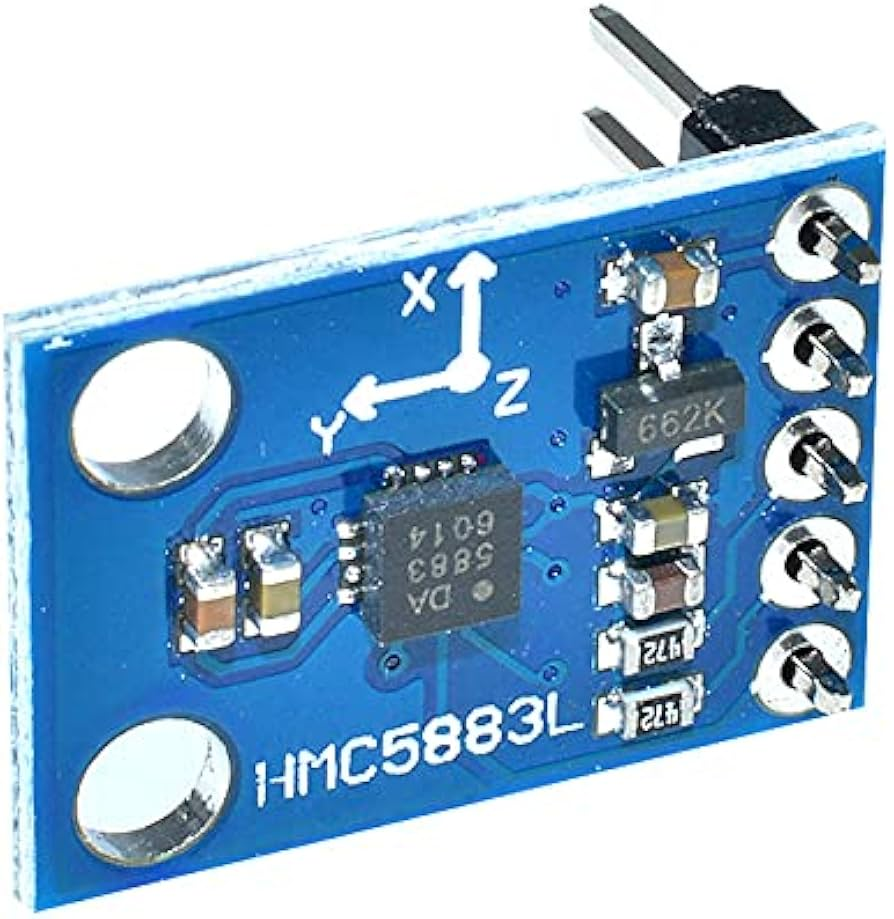
\includegraphics[width=0.2\linewidth]{img/magneto}
	
	\vspace{2mm} % Espacio entre imagen y descripción
	
	\textbf{Figura 41:} Magnetómetro
\end{center}

\vspace{5mm} % Espacio entre imágenes

% Segunda imagen con su descripción
\begin{center}
	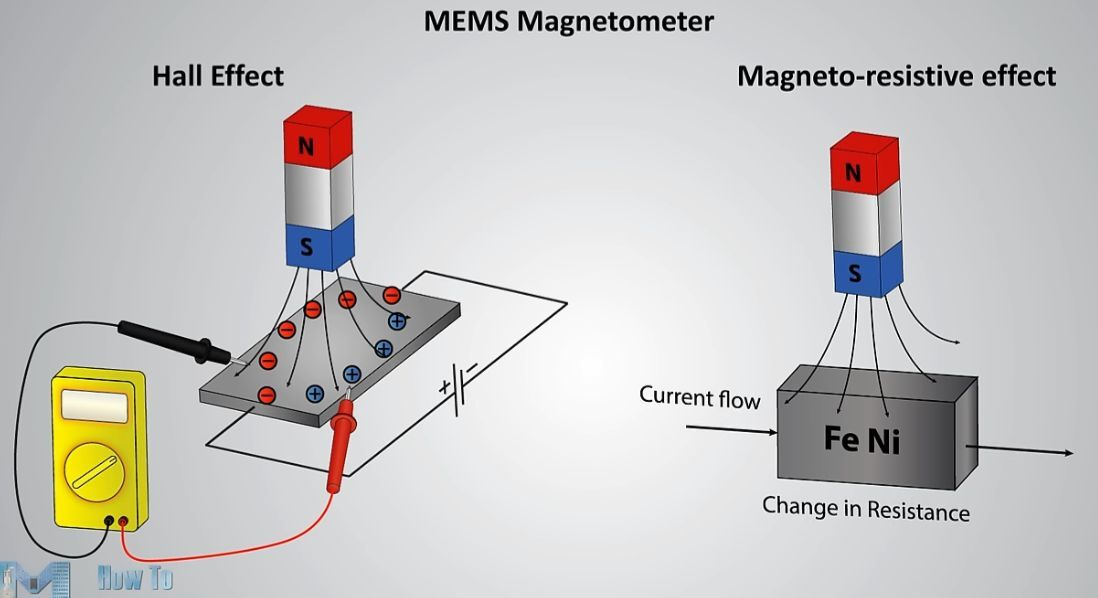
\includegraphics[width=0.6\linewidth]{img/Smagnometro}
	
	\vspace{2mm} % Espacio entre imagen y descripción
	
	\textbf{Figura 42:} Funcionamiento del magnetómetro
\end{center}


\vspace{10mm}
\textbf{LiDAR:}
La tecnología LiDAR se emplea para crear mapas topográficos detallados y modelos 3D precisos, esenciales para la navegación de vehículos autónomos en entornos dinámicos. También se utiliza en la evaluación de riesgos naturales, como flujos de lava, deslizamientos de tierra, tsunamis e inundaciones.
Un sistema LiDAR típico consta de varios componentes:
Un escáner láser que emite pulsos de luz láser en el espectro casi infrarrojo.
Un sensor LiDAR que detecta y captura los pulsos reflejados.
Un procesador que calcula el tiempo y la distancia para construir la nube de puntos LiDAR resultante.
Para lograr una medición precisa, el sistema también incorpora componentes adicionales como electrónica de cronometraje, una unidad de medición inercial (IMU) y un GPS.
\vspace{10pt}  % Espacio de 10 puntos

% Espacio para evitar que LaTeX mueva imágenes
\vspace{5mm}

% Imagen con su descripción
\begin{center}
	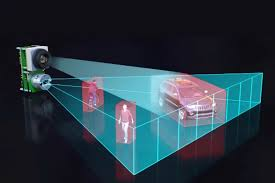
\includegraphics[width=0.3\linewidth]{img/lidar}
	
	\vspace{2mm} % Espacio entre imagen y descripción
	
	\textbf{Figura 43:} Sensor LiDAR
\end{center}
\newpage  % Salto de página forzado



\section{Tablas}
Existen varias formas de crear tablas además de este entorno, como \texttt{array}, \texttt{longtable} y \texttt{tabularx}, que permiten manejar datos extensos de manera eficiente. También es posible convertirlas desde páginas, como en \href{https://tableconvert.com/es/excel-to-latex}{TableConvert}, que permite transformar datos de Excel a formato \LaTeX fácilmente.

A continuación, se presenta una tabla larga como ejemplo:

\newcounter{actividad} % Define un contador llamado "actividad"
\begin{longtable}{|c|p{10cm}|c|} % Define anchos específicos
	\caption{Ejemplo de Tabla Larga.} \label{tab:ejemplo_tabla} \\
	\hline
	\textbf{No.} & \textbf{Descripción} & \textbf{Estado} \\
	\hline
	\endfirsthead
	\multicolumn{3}{c}{{\tablename\ \thetable{} -- continuación}} \\
	\hline
	\textbf{No.} & \textbf{Descripción} & \textbf{Estado} \\
	\hline
	\endhead
	\hline \multicolumn{3}{r}{{Continúa en la siguiente página...}} \\
	\hline
	\endfoot
	\hline
	\endlastfoot
	% Contenido de la tabla
	1 & Lorem ipsum dolor sit amet, consectetur adipiscing elit. & Completado \\
	2 & Sed do eiusmod tempor incididunt ut labore et dolore magna aliqua. & En proceso \\
	3 & Ut enim ad minim veniam, quis nostrud exercitation ullamco laboris. & Pendiente \\
	4 & Duis aute irure dolor in reprehenderit in voluptate velit. & Pendiente \\
	5 & Excepteur sint occaecat cupidatat non proident. & Pendiente \\
	6 & Sunt in culpa qui officia deserunt mollit anim id est laborum. & Pendiente \\
	7 & Curabitur pretium tincidunt lacus, nulla gravida orci a odio. & Pendiente \\
	8 & Nullam varius, turpis et commodo pharetra. & Pendiente \\
	9 & Sed ac orci quis tortor imperdiet venenatis. & Pendiente \\
	10 & Duis eget orci sit amet orci dignissim rutrum. & Pendiente \\
	11 & Nam dui ligula, fringilla a, euismod sodales, sollicitudin vel, wisi. & Pendiente \\
	12 & Pellentesque habitant morbi tristique senectus et netus et malesuada. & Pendiente \\
	13 & Fusce convallis metus id felis luctus adipiscing. & Pendiente \\
	14 & Pellentesque dapibus hendrerit tortor. & Pendiente \\
	15 & Praesent egestas tristique nibh. & Pendiente \\
	16 & Curabitur a felis in nunc fringilla tristique. & Pendiente \\
	17 & Phasellus nec sem in justo pellentesque facilisis. & Pendiente \\
	18 & Etiam imperdiet imperdiet orci. & Pendiente \\
	19 & Vestibulum ante ipsum primis in faucibus orci luctus et ultrices. & Pendiente \\
	20 & Quisque id mi. Integer ante arcu, accumsan a, consectetuer eget, posuere ut, mauris. & Pendiente \\
\end{longtable}
\section{Ecuaciones}
Para realizar ecuaciones, se pueden ayudar mucho de ChatGPT (Como copiar una imagen y que lea la ecuación para dártela en formato \LaTeX) y de que MATLAB, word y algunas páginas te permiten copiar ecuaciones en formato \LaTeX. El modelo en espacio de estados de un robot de dos grados de libertad, el cual se puede ver en el Capítulo 5: Dinámica del Robot en \cite{barrientos2007fundamentos} se expresa como

\begin{equation}
	\label{eq:spaceStateRobot}
	\begin{bmatrix}
		\dot{q} \\
		\ddot{q}
	\end{bmatrix} =
	\begin{bmatrix}
		0 & I \\
		M^{-1}(-C - G)
	\end{bmatrix}
	\begin{bmatrix}
		q \\
		\dot{q}
	\end{bmatrix} +
	\begin{bmatrix}
		0 \\
		M^{-1} B
	\end{bmatrix} u,
\end{equation}
donde:
\begin{itemize}
	\item \( q \) es el vector de posiciones articulares del robot.
	\item \( \dot{q} \) y \( \ddot{q} \) son las velocidades y aceleraciones articulares.
	\item \( M \) es la matriz de inercia.
	\item \( C \) representa las fuerzas centrífugas y de Coriolis.
	\item \( G \) es el vector de fuerzas gravitacionales.
	\item \( B \) es la matriz de entrada de los torques.
	\item \( u \) es el vector de torques aplicados a las articulaciones.
\end{itemize}

Cabe destacar que en \eqref{eq:spaceStateRobot}, la ecuación se referencia después de haberla nombrado y forma parte de la oración, por lo que debe llevar puntos o comas. También al referenciar, debe de estar entre paréntesis con \texttt{eqref}.
\section{Conclusión} \label{sec:conclusion}

Durante la elaboración de este trabajo nos enfrentamos a diversos retos que complicaron nuestro trabajo, siendo el más grande el comprender y aprender a utilizar la herramientas de LaTex y Github. 

Al no estar familiarizados con estos entornos de programación, tuvimos problemas al comenzar a enlazarnos para colaborar en el documento sin embargo logramos aprender y realizar un buen trabajo. Otro problema que se nos presentó fue utilizar la sintaxis de LaTex, no obstante al momento de comenzar a trabajar se nos fue facilitando con la practica. 

\begin{thebibliography}{99}
	
	
	\bibitem{herga} 
	HERGA. (2020). 
	\textit{¿Qué es un interruptor neumático?}. Recuperado el 14 de febrero de 2025 de \url{https://www.herga.com/news-media/technical-blog-archive/what-is-a-pneumatic-switch-}
	
	\bibitem{kolstad} 
	Kolstad, C. (2025). 
	\textit{¿Qué es un Transductor de Presión?}. TAMESON. Recuperado el 14 de febrero de 2025 de \url{https://tameson.es/pages/transductores-de-presion-como-funcionan}
	
	\bibitem{peterson} 
	Peterson, Z. (2023). 
	\textit{Dominando el magnetismo: sensores de efecto Hall y sus aplicaciones para PCB}. Altium. Recuperado el 14 de febrero de 2025 de \url{https://resources.altium.com/es/p/mastering-magnetism-hall-effect-sensors-and-applications-pcbs}
	
	\bibitem{senstar} 
	SENSTAR. (s.f.). 
	\textit{Sensores de microondas}. Recuperado el 14 de febrero de 2025 de \url{https://senstar.com/es/senstarpedia/sensores-de-microondas/#:~:text=Los%20sensores%20de%20microondas%20utilizan,el%20principio%20del%20efecto%20Doppler}
	
	\bibitem{keyence1} 
	KEYENCE. (s.f.). 
	\textit{¿Qué es un sensor ultrasónico?}. Recuperado el 14 de febrero de 2025 de \url{https://www.keyence.com.mx/ss/products/sensor/sensorbasics/ultrasonic/info/}
	
	\bibitem{keyence2} 
	KEYENCE. (s.f.). 
	\textit{¿Qué es un sensor láser de tipo de reconocimiento de “luz recibida”?}. Recuperado el 14 de febrero de 2025 de \url{https://www.keyence.com.mx/ss/products/sensor/sensorbasics/laser_light/info/}
	
	\bibitem{keyence3} 
	KEYENCE. (s.f.). 
	\textit{¿Qué son los sensores de visión?}. Recuperado el 14 de febrero de 2025 de \url{https://www.keyence.com.mx/ss/products/sensor/sensorbasics/vision/info/}
	
	\bibitem{ridgway} 
	Ridgway, J. (2022). 
	\textit{¿Qué son los sensores de visión?}. Cognex. Recuperado el 14 de febrero de 2025 de \url{https://www.cognex.com/es-mx/blogs/machine-vision/what-are-vision-sensors}
	
	\bibitem{Saha} 
	Saha, S. K. (2008)
	\textit{Introducción a la robótica.} McGraw Hill.
	
	\bibitem{Barrientos} 
	Barrientos, A. y Peñin, L. (2007) 
	\textit{FUNDAMENTOS DE ROBÓTICA.} McGraw Hill.
	
	\bibitem{Servo} 
	Servo-user. (2025). 
	\textit{¿Cuál es la diferencia entre encoder incremental y absoluto?}Servomotors Adjust. Recuperado el 14 de febrero de 2025 de \url{https://www.servomotorsadjust.com/cual-es-la-diferencia-entre-un-encoder-incremental-y-absoluto/}

	\bibitem{Lidar} 
	IBM. (s.f.). 
	\textit{¿Qué es LiDAR?}  Recuperado el 14 de febrero de 2025 de \url{https://www.ibm.com/mx-es/topics/lidar}
	
	
\end{thebibliography}



%-------------------------------------------
% Bibliografía
%-------------------------------------------
%\bibliographystyle{IEEEtran}  % Estilo de bibliografía IEEE
% La bibliografía se tomará del archivo "fuentes.bib"
%\bibliography{fuentes}
	
\end{document}
